\documentclass{article}

% if you need to pass options to natbib, use, e.g.:
% \PassOptionsToPackage{numbers, compress}{natbib}
% before loading nips_2018

% ready for submission
\usepackage{nips_2018}
\usepackage{amsmath,amssymb}
\usepackage{calrsfs}
\usepackage[utf8]{inputenc}
\usepackage{hyperref}
\usepackage{algpseudocode}
\usepackage{algorithm}
\usepackage{comment}
\usepackage{dsfont}
\usepackage{bbm}
\usepackage{graphicx}
\usepackage[
backend=biber,
style=numeric,
sorting=none
]{biblatex}
\addbibresource{bib.bib}

% to compile a preprint version, e.g., for submission to arXiv, add
% add the [preprint] option:
% \usepackage[preprint]{nips_2018}

% to compile a camera-ready version, add the [final] option, e.g.:
% \usepackage[final]{nips_2018}

% to avoid loading the natbib package, add option nonatbib:
% \usepackage[nonatbib]{nips_2018}

\usepackage[utf8]{inputenc} % allow utf-8 input
\usepackage[T1]{fontenc}    % use 8-bit T1 fonts
\usepackage{hyperref}       % hyperlinks
\usepackage{url}            % simple URL typesetting
\usepackage{booktabs}       % professional-quality tables
\usepackage{amsfonts}       % blackboard math symbols
\usepackage{nicefrac}       % compact symbols for 1/2, etc.
\usepackage{microtype}      % microtypography
\usepackage{graphicx}
\usepackage{authblk}
\title{Real-Time Backfill Correction of COVID-19 Infections
}

% The \author macro works with any number of authors. There are two
% commands used to separate the names and addresses of multiple
% authors: \And and \AND.
%
% Using \And between authors leaves it to LaTeX to determine where to
% break the lines. Using \AND forces a line break at that point. So,
% if LaTeX puts 3 of 4 authors names on the first line, and the last
% on the second line, try using \AND instead of \And before the third
% author name.

\author{Jingjing Tang, Roni Rosenfeld}

\begin{document}
% \nipsfinalcopy is no longer used

\maketitle

\begin{abstract}


\end{abstract}


\section{Introduction}

As a global public health issue resulting in extreme societal, economic, and political disruption, the COVID-19 pandemic has highlighted the importance of proactive epidemic forecasting, critical in providing response guidance for policymakers and healthcare authorities. However, the latency problem commonly exists in public health surveillance data streams. It often causes imperfect or even error-prone situational awareness \cite{McGough2020}\cite{Rosenfeld2021} and brings challenges to real-time forecasting accuracy. 

To be more detailed, the latency problem refers to the situation where the observations or statistics provided by the surveillance systems are most up-to-date but not finalized. The initially released data is usually revised/corrected through a process known as the \textit{backfill} phenomenon. Except for errata, some data will only be reported once with some degree of reporting delay, which is regarded as a special case of backfill. The term \textit{backfill correction} we used throughout this paper refers to providing projection of finalized values based on the current observations.

Many factors can affect the magnitude of backfill, such as laboratory confirmation, infrastructure difficulties, coordination efficiency between health authorities and government\cite{reich2019collaborative}\cite{Chakraborty2018}, etc. Understanding the backfill pattern is crucial, as it could lead to intelligent strategies for making accurate projection of the observations that are far from finalized. Backfill has been commonly mentioned in public health studies, ranging from influenza\cite{chakraborty2018know}, dengue\cite{rangarajan2019forecasting} to COVID-19 forecasting\cite{rodriguez2021deepcovid}. Different approaches have been proposed to address the backfill problem retrospectively and in real time. One common strategy is to re-scale real-time reports by estimating scaling factors from historical data\cite{lawless1994adjustments}\cite{hohle2014bayesian}. Other ones such as backcasting handle the reporting error by generating past weeks’ validation data using the most recent data reports for those weeks and accounting for uncertainty in reporting patterns\cites{brooks2018nonmechanistic}. Nowcasting studies deal with backfill via complicated statistical or machine learning methods\cite{li2021bayesian}\cite{mjahja2021} strictly based on incomplete data. 

It is worth noting that backfill correction is more challenging for COVID-19 from two perspectives: 1) SARS-CoV-2 is constantly changing, and the dominant variant is continuously updated while the epidemic pattern of seasonal influenza is more stable and less noisy; 2) the degree of concern and response measures from the government and healthcare authorities to COVID-19 is constantly changing as well, making the pattern of data collation and revision difficult to predict. Despite this, digital surveillance, developed in the recent years especially during the COVID-19 pandemic, play an indispensable role in understanding and modeling backfill patterns. Data revision history is no longer ignored but well captured and archived with support of new technology and methods.


In this paper, we focus on making projection of the finalized values of observations in \textit{real-time} and measuring the uncertainty in projection, laying out a framework for an operational backfill correction system using provisional data. At any given date $s$, we are forced to use data that is guaranteed to be available at date $s$. Specifically, backfill correction takes as input all the revisions of observations with finalized values included as the target, and output the estimation of probability distribution over the target variable based on the most up-to-date observations. There are two categories of observations that we mainly care about: 1) counts; 2) fractions. Take COVID-19 insurance claims data as an example, counts can be the number of outpatient insurance claims that's made for COVID-19 patients while fractions can be the percentage of COVID outpatient insurance claims in terms of total outpatient insurance claims.

An outline for this paper is as follows. In Section 2, we provide preliminary information about notations and the problem setup. The details of the model are described in Section 3. Section 4 covers evaluation of the results and comparing the backfill correction results made in real-time to those without correction. In Section 5, we conclude with a discussion and describe a few directions for future work.


\begin{figure}
    \centering
    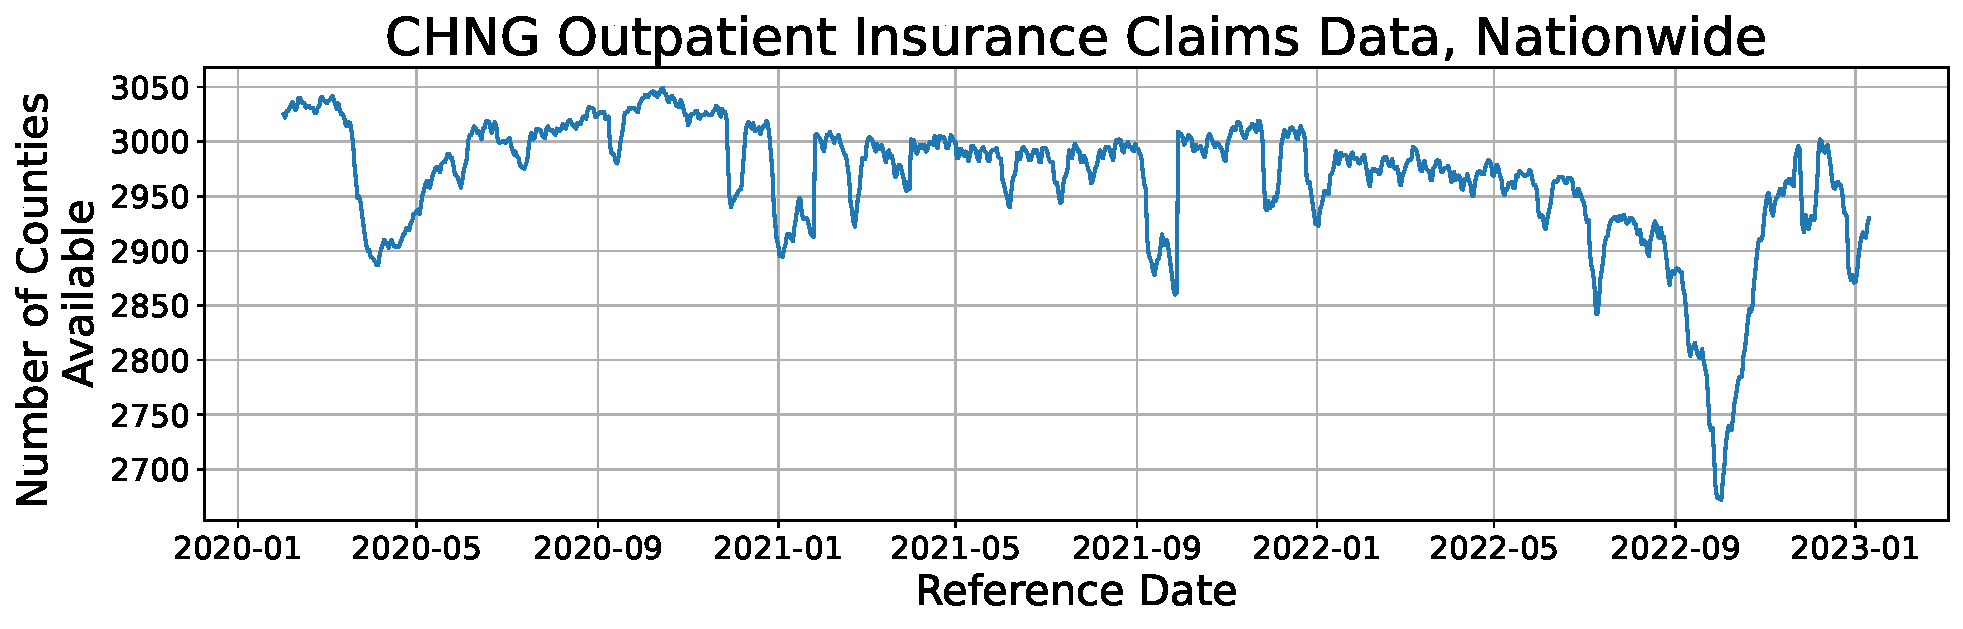
\includegraphics[width=\textwidth]{figs/available_counties.pdf}
    \caption{\textit{}}
\end{figure}

\section{Preliminaries}
Given $y_{it}$ an epidemic observation that have onset at time $t$ for location $i$, $y_{i,1:t}$ is the time series observations of the uni-variate surveillance. Due to the existence of backfill, each $y_{it}$ has its \textit{backfill sequence}\cite{kamarthi2021back2future} $y_{it}^{t:s}$ as of date $s$ ($s \geq t$). To be clear on nomenclature, throughout this paper, we use the term \textit{reference date} for date $t$ referring to the date when the observations have onset and the term \textit{report date} for date $s$ referring to the date when the observations are reported. 

For convenience, we introduce another term lag $l$ defined as $l = s-t \in \mathbf{N}$, which is the number of days between the report date $s$ and the reference date $t$. Now we change our notation henceforth and rewrite $y_{it}^s$ as $y_{itl}$. $y_{itl}$ is also named to be the $(l+1)$th release of $y_{it}$. The backfill sequence $y_{it}^{t:s}$ is equivalent to $y_{it,0:l}$. 

\begin{figure}
    \centering
    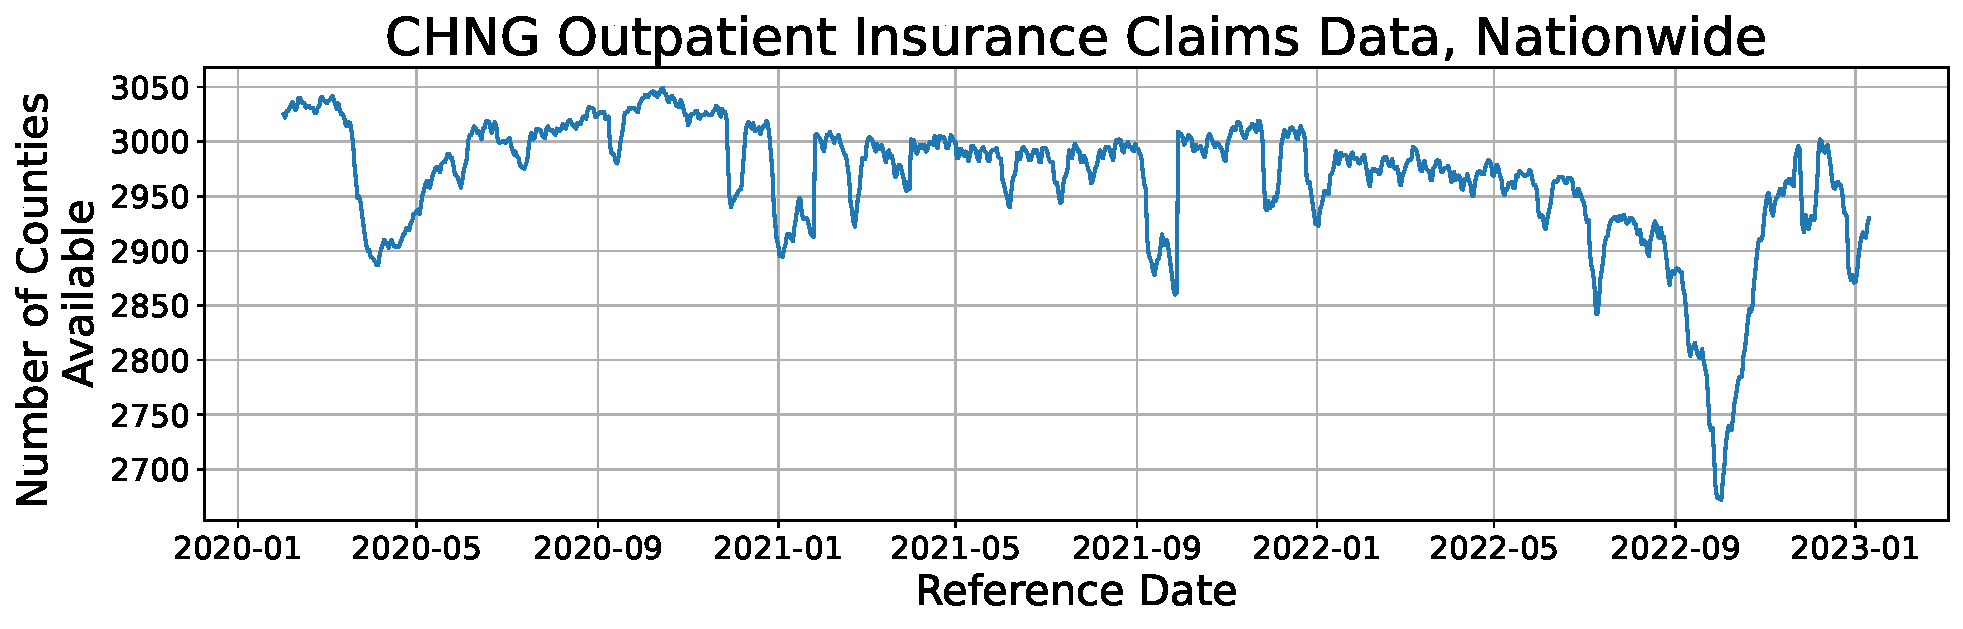
\includegraphics[width=\textwidth]{figs/available_counties.pdf}
    \caption{\textit{}}
\end{figure}


% TODO: Make the ticks larger
\begin{figure}
    \centering
    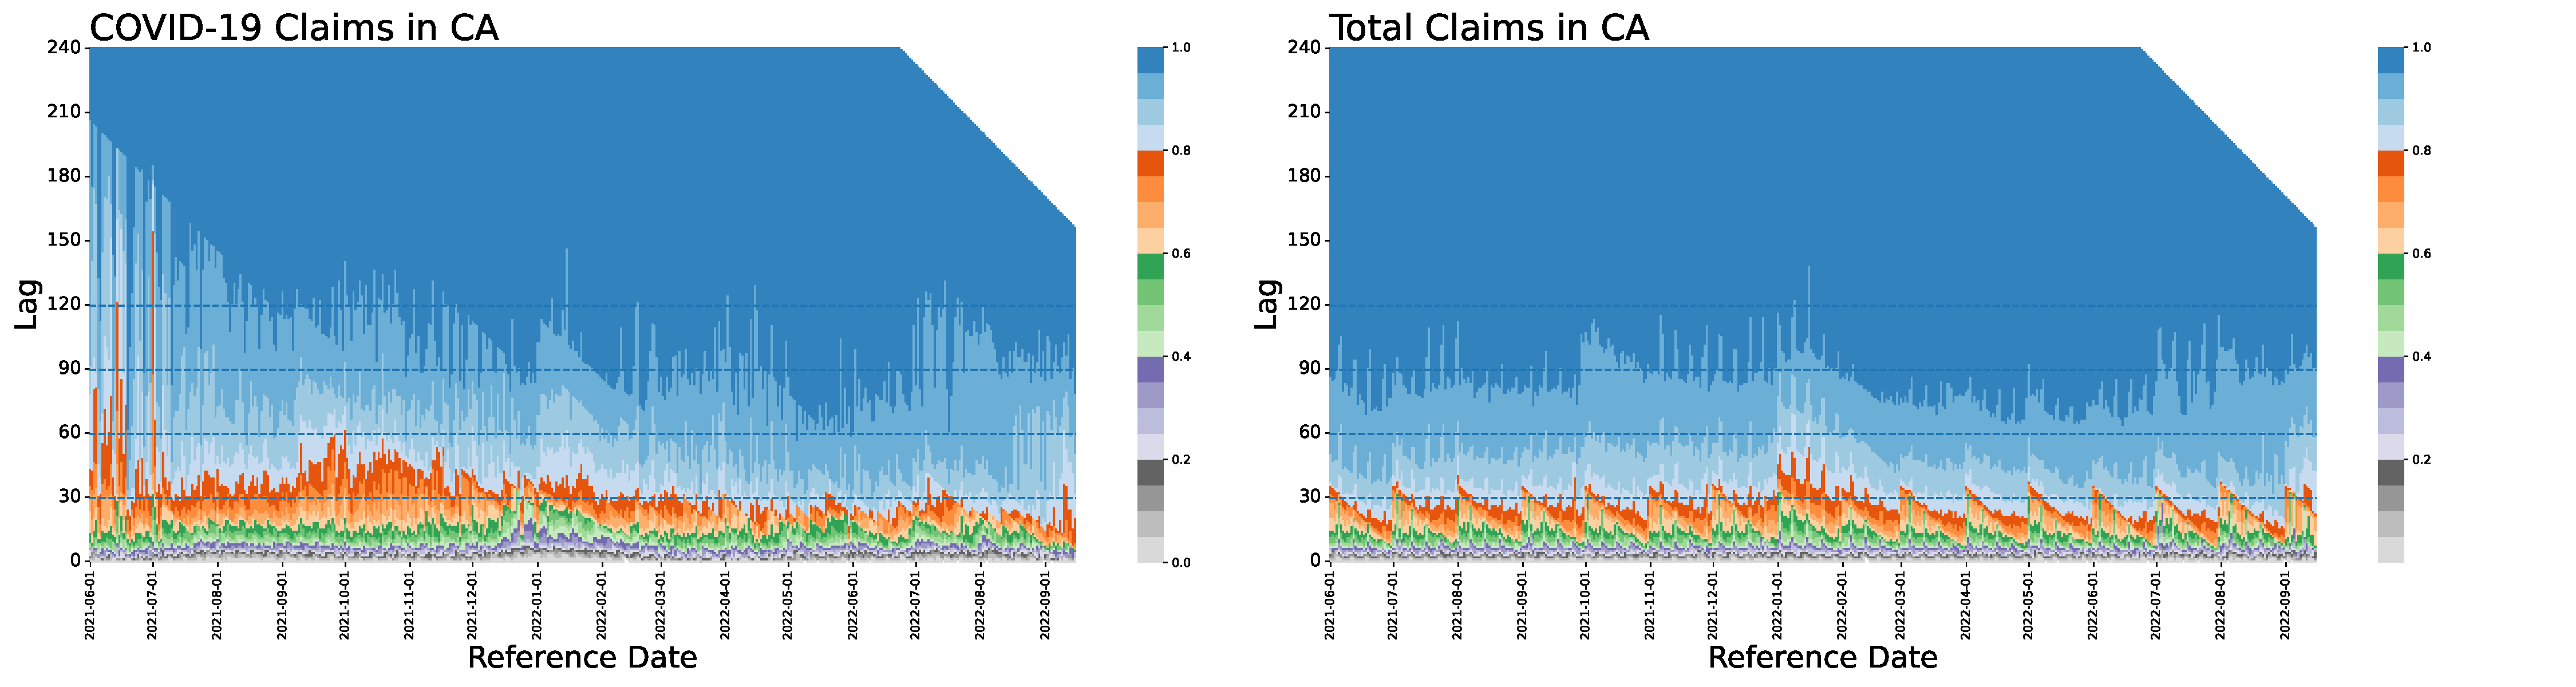
\includegraphics[width=\textwidth]{figs/completeness_CA.pdf}
    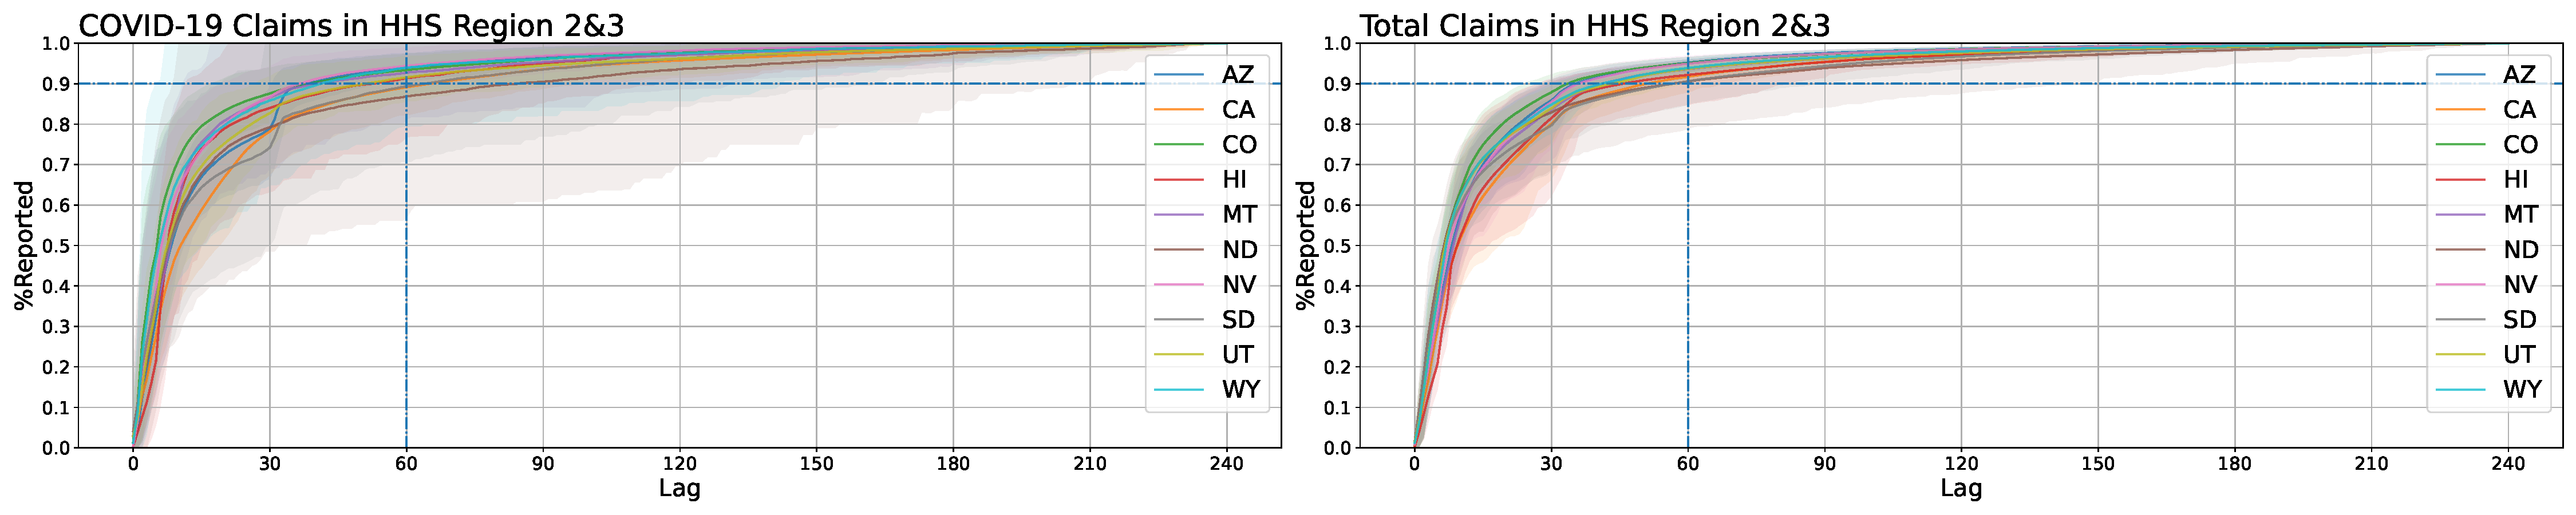
\includegraphics[width=\textwidth]{figs/completeness_lineplot_hhs8&9.pdf}
    \caption{\textit{Top: percentage of reported distribution in New York, grouped by lag, and recorded over reference dates. Bottom: Mean percentage of reported, averaged over all reference dates between 2021-04-01 and 2023-01-10, over lags for states in HHS Region 2\&3. The shaded bands correspond to 5\% quantile to 95\% quantile intervals. The left panel in the figure is based on CHNG outpatient COVID-19 claims data while the right panel is based on CHNG outpatient total claims data.}}
\end{figure}

Only a tiny part of data revisions occurs when data is lost but found later or when data is entered incorrectly but changed later. Most of them are caused by reporting delays. Therefore, the backfill sequence $y_{it,0:l}$ is guaranteed to converge to a particular value $Y_{it}$ when $l \geq L_{it}, L_{it}$ is sufficiently large. $Y_{it}$ is called the finalized value of $y_{it}$.

In this paper, we mainly use Change HealthCare (CHNG) 's insurance claims data which is available for more than two thousand most populous US counties, accounting for more than 45\% of the U.S. population in general. Multiple pre-processed signals based on this data are publicly available through Delphi's COVIDcast API \cite{reinhart2021open}. In order to construct the raw backfill data (including all historical versions), we start from the restricted line-level de-identified outpatient insurance claims data. It is worth pointing out that the data has geographic details down to 5-digit ZipCode level and is updated on a daily basis with no latency. We assume that a missing report is the same as reporting 0.

A useful way we propose to look at backfill pattern is by examining the variable $p_{itl}$ defined as $$p_{itl} = \frac{y_{itl}}{Y_{it}} \times 100\%$$
$p_{itl}$ describes the percentage of claims that have been reported after the $(l+1)$th release for location $i$ and reference date $t$. Since $Y_{it}$ is a theoretical value which is not obtainable directly, we use $y_{it}^s$ ($s$ = 2023-03-11) to approximate it. 

The distribution of $p_{itl}$ exhibiting how the backfill sequences vary over time. The day-of-week effect and week-of-month effect are evident, since the revision trends in lags for a fixed level of \%reported show spikes and bumps upward at the end of each week and around the beginning of each month. The reporting delay is prominent during the time period when the epidemic curve is at its peak. The top panel in Figure X displays results to this end using data in New York as an example. The backfill pattern is much more stable over time for total claims compared to COVID-19 claims. Overall, COVID-19 reporting is less efficient than Non-COVID-19 reporting. The variance is larger in the backfill pattern of COVID-19 claims which increases the diffculty in backfill correction. 

Furthermore, there is a high degree of heterogeneity in the backfill pattern across locations. For most of the locations (states and populous counties), the data revision tends to occur in the first two weeks of the backfill sequences to a large extent. The bottom panel in the figure shows that nearly all the mean \%reported of COVID-19 reaches 90\% when lag equals to 60 for states in HHS Region 2 and Region 3 except New Jersey. 


\subsection{Defining the Target}
Theoretically, the limit values of the backfill sequences are the target to be projected. However, the practice suggests that $L_{it}$ is highly inconsistent for different reference dates and can be incredibly large. Figure X gives an illustration where most of the states require more than 180 days (around half a year) for the backfill sequences of the COVID-19 claims reports with reference date=2021-08-01 to converge. If we set the projection target to be $Y_{it}$, we are forced to use the backfill sequences of $y_{it}$ with $t \leq s-L_{it}$ only for the training data on each testing date $s$. This means the backfill pattern captured based on the empirical distribution of all available data is very likely to be biased against the most recent backfill pattern, as discussed in the previous subsection. Note that, though $L_{it}$ is far from uniform at random, the distribution of \%reported indicates that substantial effective revisions are usually made within the first two months. Thus, we step back, setting a target lag $L$ and using $Y_{itL}$ as the projection target. For any location $i$ and reference date $t$, we assume that $$\mathbf{E}[\frac{Y_{itL} - Y_{it}}{Y_{it}}] \leq \epsilon $$ The larger the target lag $L$ is, the smaller $\epsilon$ can be. In short, the target lag $L$ selection faces a trade-off between timeliness and accuracy. Out of practical considerations and understanding of CHNG outpatient data, we set $L=60$ henceforth in our real-time backfill correction experiments.

\begin{figure}
    \centering
    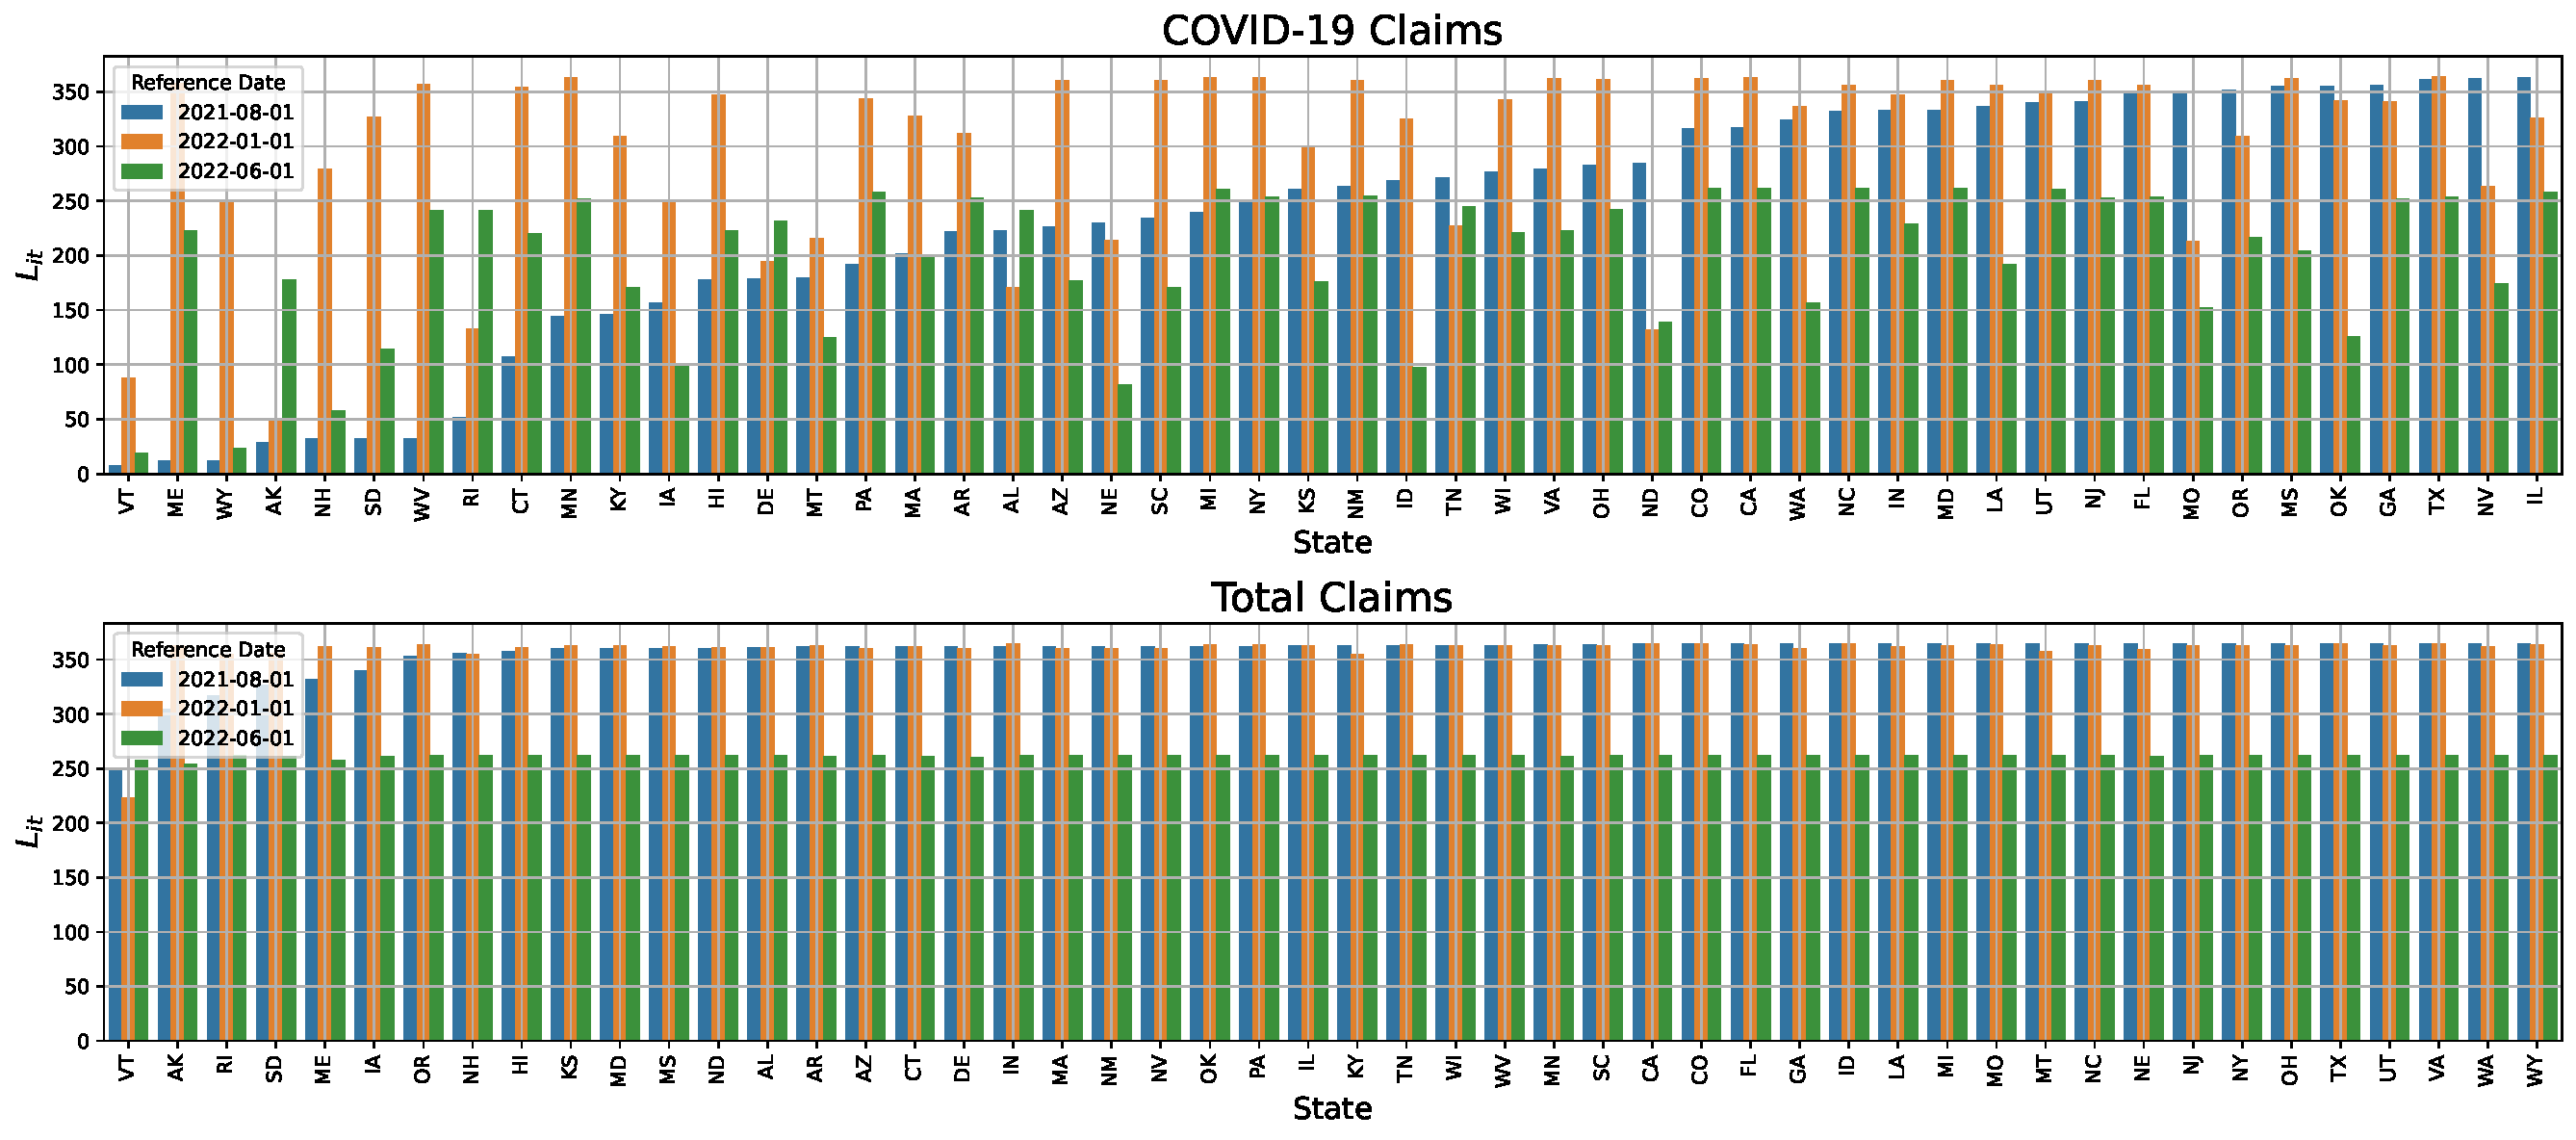
\includegraphics[width=\textwidth]{figs/Lit_examples.pdf}
    \caption{\textit{Top: comparison of the smallest lags required for convergence across states, displayed for a sample of different reference dates, based on CHNG outpatient COVID-19 claims data. Bottom: as in the figure on the top, but based on CHNG outpatient total claims data.}}
\end{figure}

\subsection{Problem Setup}
\textit{Estimation Period}. For every report day $t$ in between 2021-08-30 and 2023-03-11 inclusive (589 days in total), we make projections of the indicator values of reference dates $t, t-1, t-2, \cdots, t-(L-1)$ respectively based only on the data that would have been available as of time $t$. 

\textit{Geographic Scope}. We produce quantile projections for the targets of each reference date at state resolution and additionally produce the estimates for the top 200 populous U.S. counties. 

\textit{Evaluation}. We evaluate all the quantile projections in between 2021-06-01 and 2023-01-10 inclusive (589 days in total) and at each of the locations (50 states and 200 counties) against the target values as defined in section 2.1.


   
\section{Methods}
In this section, we propose a non-parametric model based on quantile regression to model backfill patterns and introduce the covariates that help capture the backfill dynamics across time. 

\subsection{Real-Time Quantile Regression}

For any test date $S$, we are trying to make distributional projection of $Y_{itL}$ for all $t \in [S-L, S)$. We use the notation $Q_{Y_{itL}|X_{itl}}^{\tau}$ to represent the $\tau$th quantile of $Y_{itL}$ given $X_{itl}$, where $X_{itl}$ is the vector of features based on $\{y_{itl}\}_{t+l\leq s}$. 
$$Q_{Y_{itL}|X_{itl}}^{\tau} = \inf \{y: F_{Y_{itL}|X_{itl}}(y) \geq \tau\}$$
Motivated by reducing the relative error between the projections and the target, we do a log transformation (natural logarithm) $f(x) = log(x + a)$ of all the variables. $a$ is a small enough constant to avoid invalid values. Since $f(\cdot)$ is monotonically increasing, 
$$ Q_{f(Y_{itL})|X_{itl}}^{\tau} = f(Q_{Y_{itL}|X_{itl}}^{\tau}) $$
We now make the assumption that the $\tau$th conditional quantile on log scale is given as a linear function of explanatory variables.

$$Q_{f(Y_{itL})|f(X_{itl})}^{\tau}= \beta^{\tau T}X_{itl}$$
The covariates included in $X_{itl}$ are the following:
\begin{itemize}
    \item $\mathbbm{1}(\mbox{wd}(t+l) == k)$: indicator functions checking the day-of-week of the report date $t+l$, where $k \in \{0, 1, 2, ..., 5\}$. 
    \item $\mathbbm{1}(\mbox{wd}(t) == k)$ : indicator functions checking the day-of-week of the report date $t$, where $k \in \{0, 1, 2, ..., 5\}$.
    \item $\mathbbm{1}(\mbox{mw}(t+l) == k)$ : indicator functions checking the week-of-month of report date $t+l$, where $k \in \{0, 1, 2, ...,3\}$
    \item $f(\widetilde{y}_{itl})$: average of 7-day past values on log scale.
    \item $\mathbbm{1}(\sqrt{y_{itl}} \in \mbox{interval}_k)$ where $\mbox{interval}_k$ are uniform bins at square-root level
    \item \mbox{7day-slope}: $f(\widetilde{y}_{itl}) - f(\widetilde{y}_{i(t-7)(l+7)})$ : the 7-day slope, where we compare the difference between the 7-day average of current observations and the 7-day average of the observation assigned to 7 days ago on log scale.
    \item 7day-Modification where we compare the difference between the 7-day average of the current raw counts and the 7-day average from the first release. 
    $$\mbox{7day-Mod} = f( \widetilde{y}_{itl}) - f(\widetilde{y}_{it0})$$
    \item 7day-Prev-Mod-start where we compare the difference between the 7-day average of the raw counts reported a week ago with the same lag and the 7-day average of the raw counts reported a week ago from the first release. 
    $$\mbox{7day-Prev-Mod-Start} = f( \widetilde{y}_{i(t-7)l}) - f(\widetilde{y}_{i(t-7)0})$$
    \item 7day-Prev-Mod-follow 
    $$\mbox{7day-Prev-Mod-Follow} = f(\widetilde{y}_{i(t-7)l}) - f( \widetilde{y}_{i(t-7)(l+7)})$$

\end{itemize}
$\mbox{wd}(\cdot)$ is a function returning the day of the week as integers, where Monday is 0 and Sunday is 6. $\mbox{mw}(\cdot)$ is a function checking the week of a month. For example, $\mbox{mw}(\cdot) = 0$ represents the first week of a month that starts from a Sunday. $\widetilde{y}_{itl} = \sum_{v=1}^7 y_{i(t-v)(l+v)}$ is the average of 7-day past values reported at the same date $t+l$

We achieve the estimates of coefficients by solving the problem
$$ \beta^{\tau} = \arg\min_{\beta} \sum_{l\in \mathcal{L}, t+l < S}(\rho_\tau (f(Y_{itL}) - X_{itl}\beta)) + \lambda ||\beta||_1$$

where $\rho$ is the quantile loss\cite{Koenker1978}, $\mathcal{L} = \{l: 0 \leq l \leq L\}$. $||\cdot||_1$ is the $\mathcal{l}_1$ norm. The hyper-parameter $\lambda \geq 0$ controls the complexity of the model. 


The model is trained adaptively. At each test date $S$, a series of new observations is reported which gives a series of $y_{itl}$s,

$$y_{i}^S = \{\underbrace{y_{i,S,0}, y_{i, (S-1), 1}, y_{i, (S-2), 2}, \cdots, y_{i, (S -L +1),(L-1)}}_\text{Testing Data}, \underbrace{y_{i, (S-L), L}}_\text{Target},  \cdots \}$$.
Note that, the backfill sequence of $y_{i(S-L)}$ is moved from testing to training since the target $y_{i,(S-L), L}$ becomes available. 

\begin{figure}
    \centering
    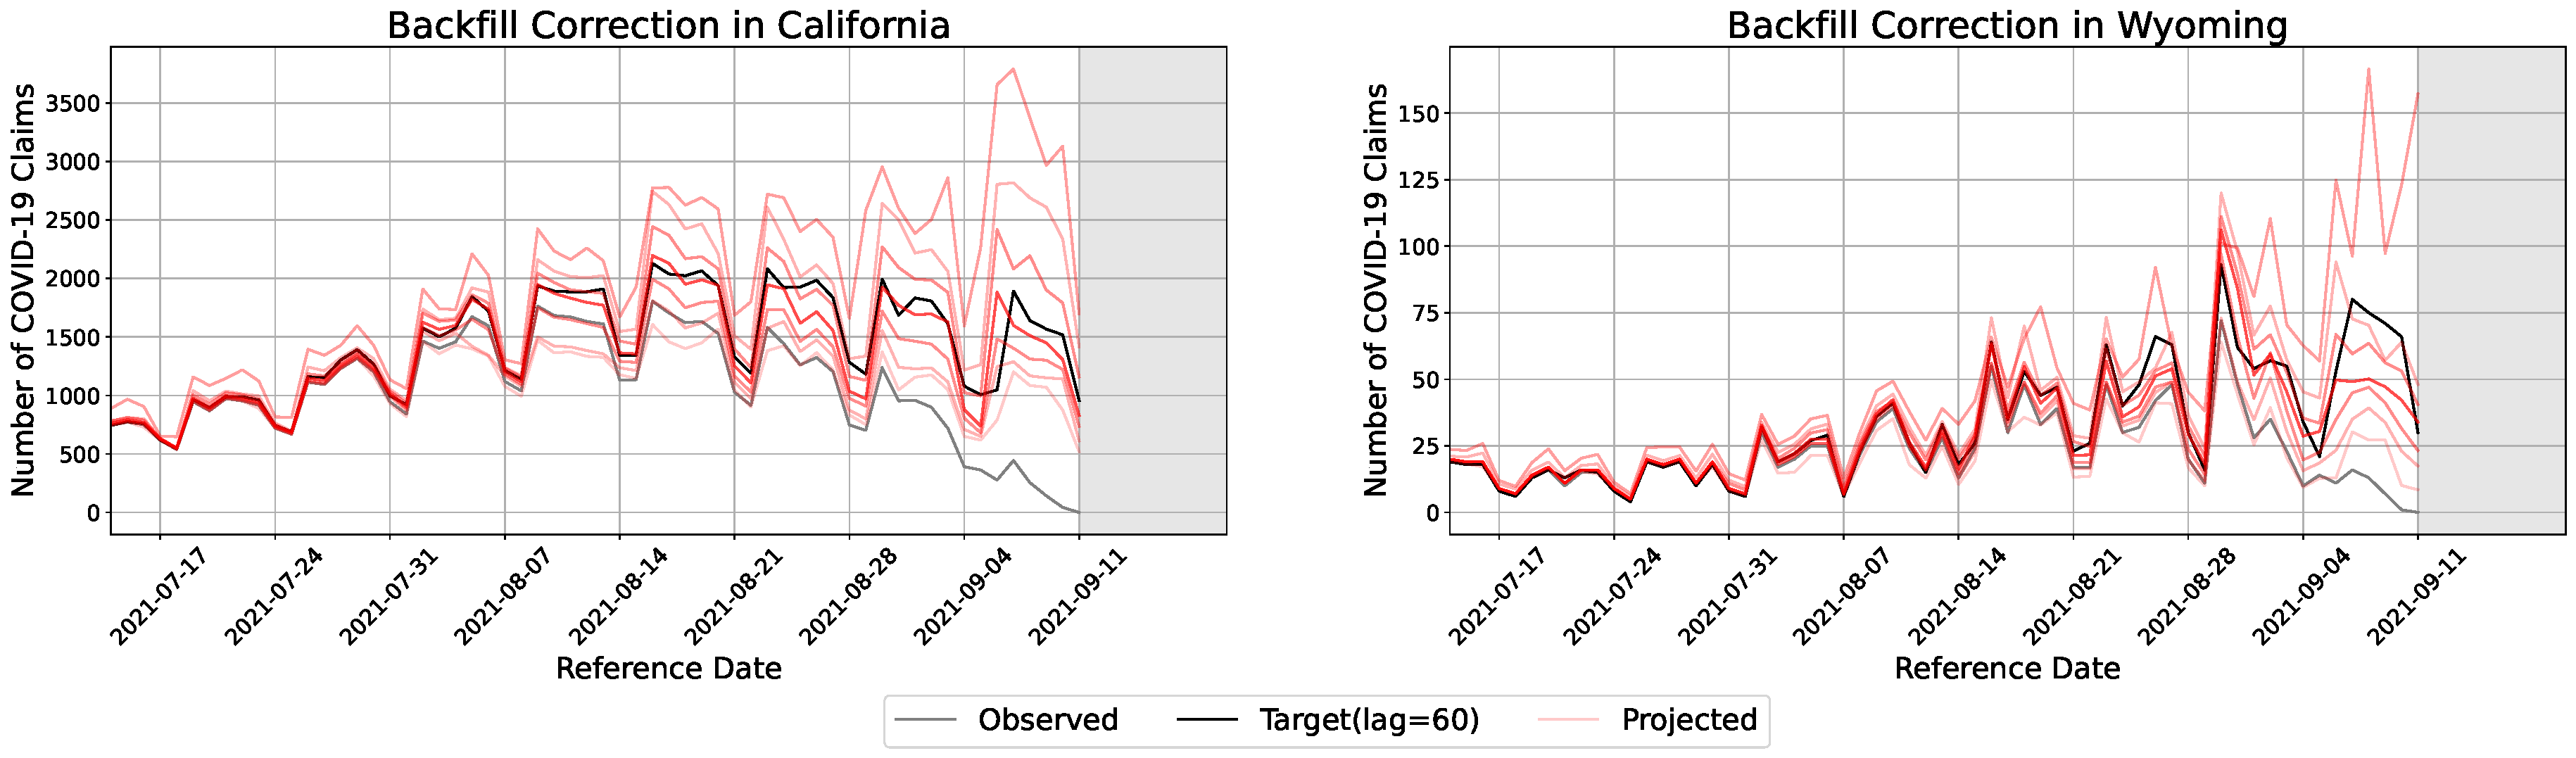
\includegraphics[width=\textwidth]{figs/count_pred_example_ca&wy.pdf}
    \caption{\textit{Illustration of estimating target number of CHNG outpatient COVID-19 claims as of 2021-09-11. The gray curve shows the most recent release of the number of COVID claims based on CHNG outpatient data in California and Wyoming. The red lines show the projected quantiles of the 60th revision of the number of COVID-19 claims for each reference date. The black curve shows the actual 60th revision for the values of each reference date in the future.}}
\end{figure}

\textbf{Shortening the Lag Window}
%% TODO: add a figure to explain it. Some kind of diagram? 
As the backfill patterns vary largely over lags, we investigate shortening the lag window in the regularized backfill correction problem and train separate models for observations with different levels of lag. Theoretically, training separate models is the same as training one model with all data pooled together but incorporating indicators to inform the level of lag (The only difference is that, fitting separately generates different variance estimates) in linear regression. However, it is not the case when lasso penalty is added for reducing the complexity of the model and rolling out extreme outliers. When making projection of $y_{itl'}$($l'$ is small enough, e.g. $l' \leq 7$), instead of using all the data as described above, we now change the problem to be
$$ \beta^{\tau} = \arg\min_{\beta} \sum_{l\in \mathcal{L}, t+l < S}(\rho_\tau (f(Y_{itL}) - X_{itl}\beta)) + \lambda ||\beta||_1$$
where $\mathcal{L}^(l') = \{l: l'-c \leq l \leq l'+ c\}$. The length lag window for this training is $2c +1$. Shortening the training window is not computationally advantageous since more models need to be trained, but the projection performance will be changed.

\textbf{Adjusting weights of Observations} The observations are not equally useful when estimating the backfill patterns. Weights are leveraged to observations as follow:
$$ \beta^{\tau} = \arg\min_{\beta} \sum_{l\in \mathcal{L}, t+l < S}w(\rho_\tau (f(Y_{itL}) - X_{itl}\beta)) + \lambda ||\beta||_1$$
where $w = \exp(-\gamma \cdot D_s \cdot D_y)$. $D_d$ and $D_y$ are two variables that affect weighting from different aspects. For each obervation $y_{itl}$, $D_d = S - (t+l)$ measures the \textit{freshness}, $D_y = \widetilde{y}_{i,(S),0} - \widetilde{y}_{itl}$ measures the similarity to the most up-to-date report. The hyper-parameter $\gamma \geq 0$ controls the additional $focus$ that we put on recent data. 

%% TODO
In general, there are three hyper-parameters to tune in practice:1) $c$ for controlling the training lag window ; 2) $\lambda$ for the lasso penalty; 3) $\gamma$ for controlling the weights of observations. Figure X1 and X2 shows the (not that confident about how to explain this part or are the figs currently good enough? )

\begin{figure}
    \centering
    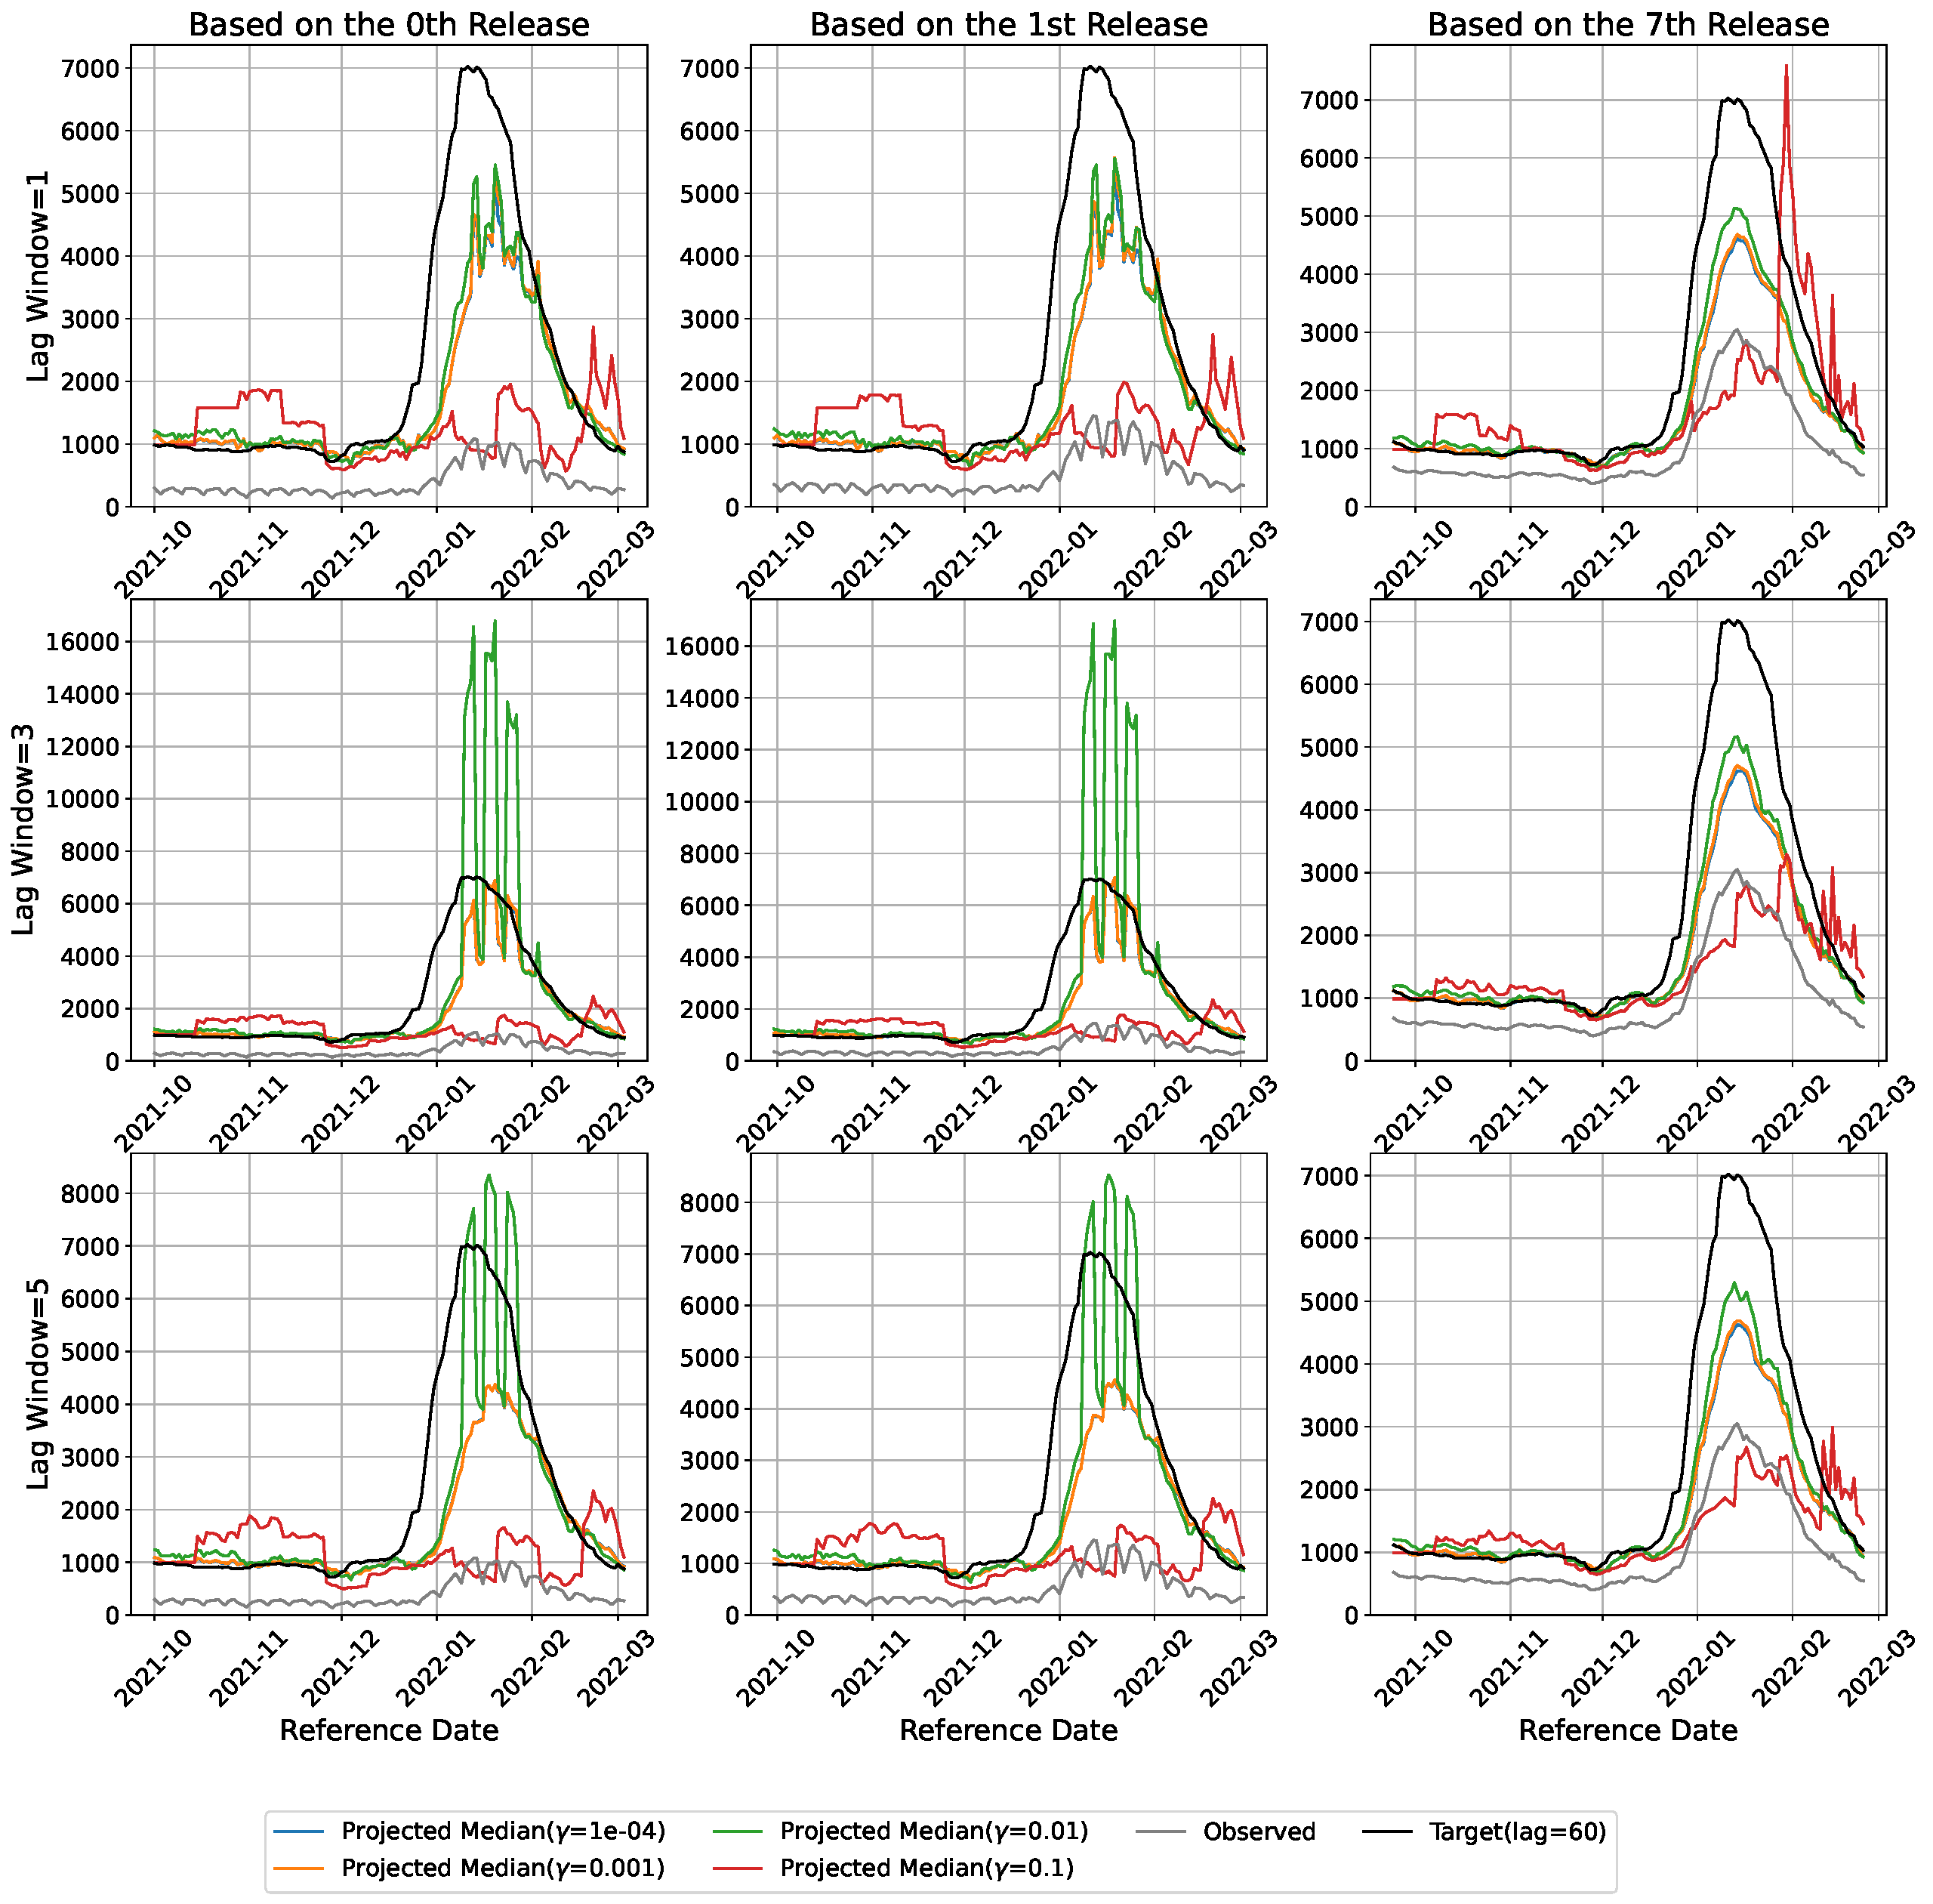
\includegraphics[width=\textwidth]{figs/count_pred_gamma_lagpad_tuning_ca_new_covs_added.pdf}
    \caption{\textit{}}
\end{figure}

\begin{figure}
    \centering
    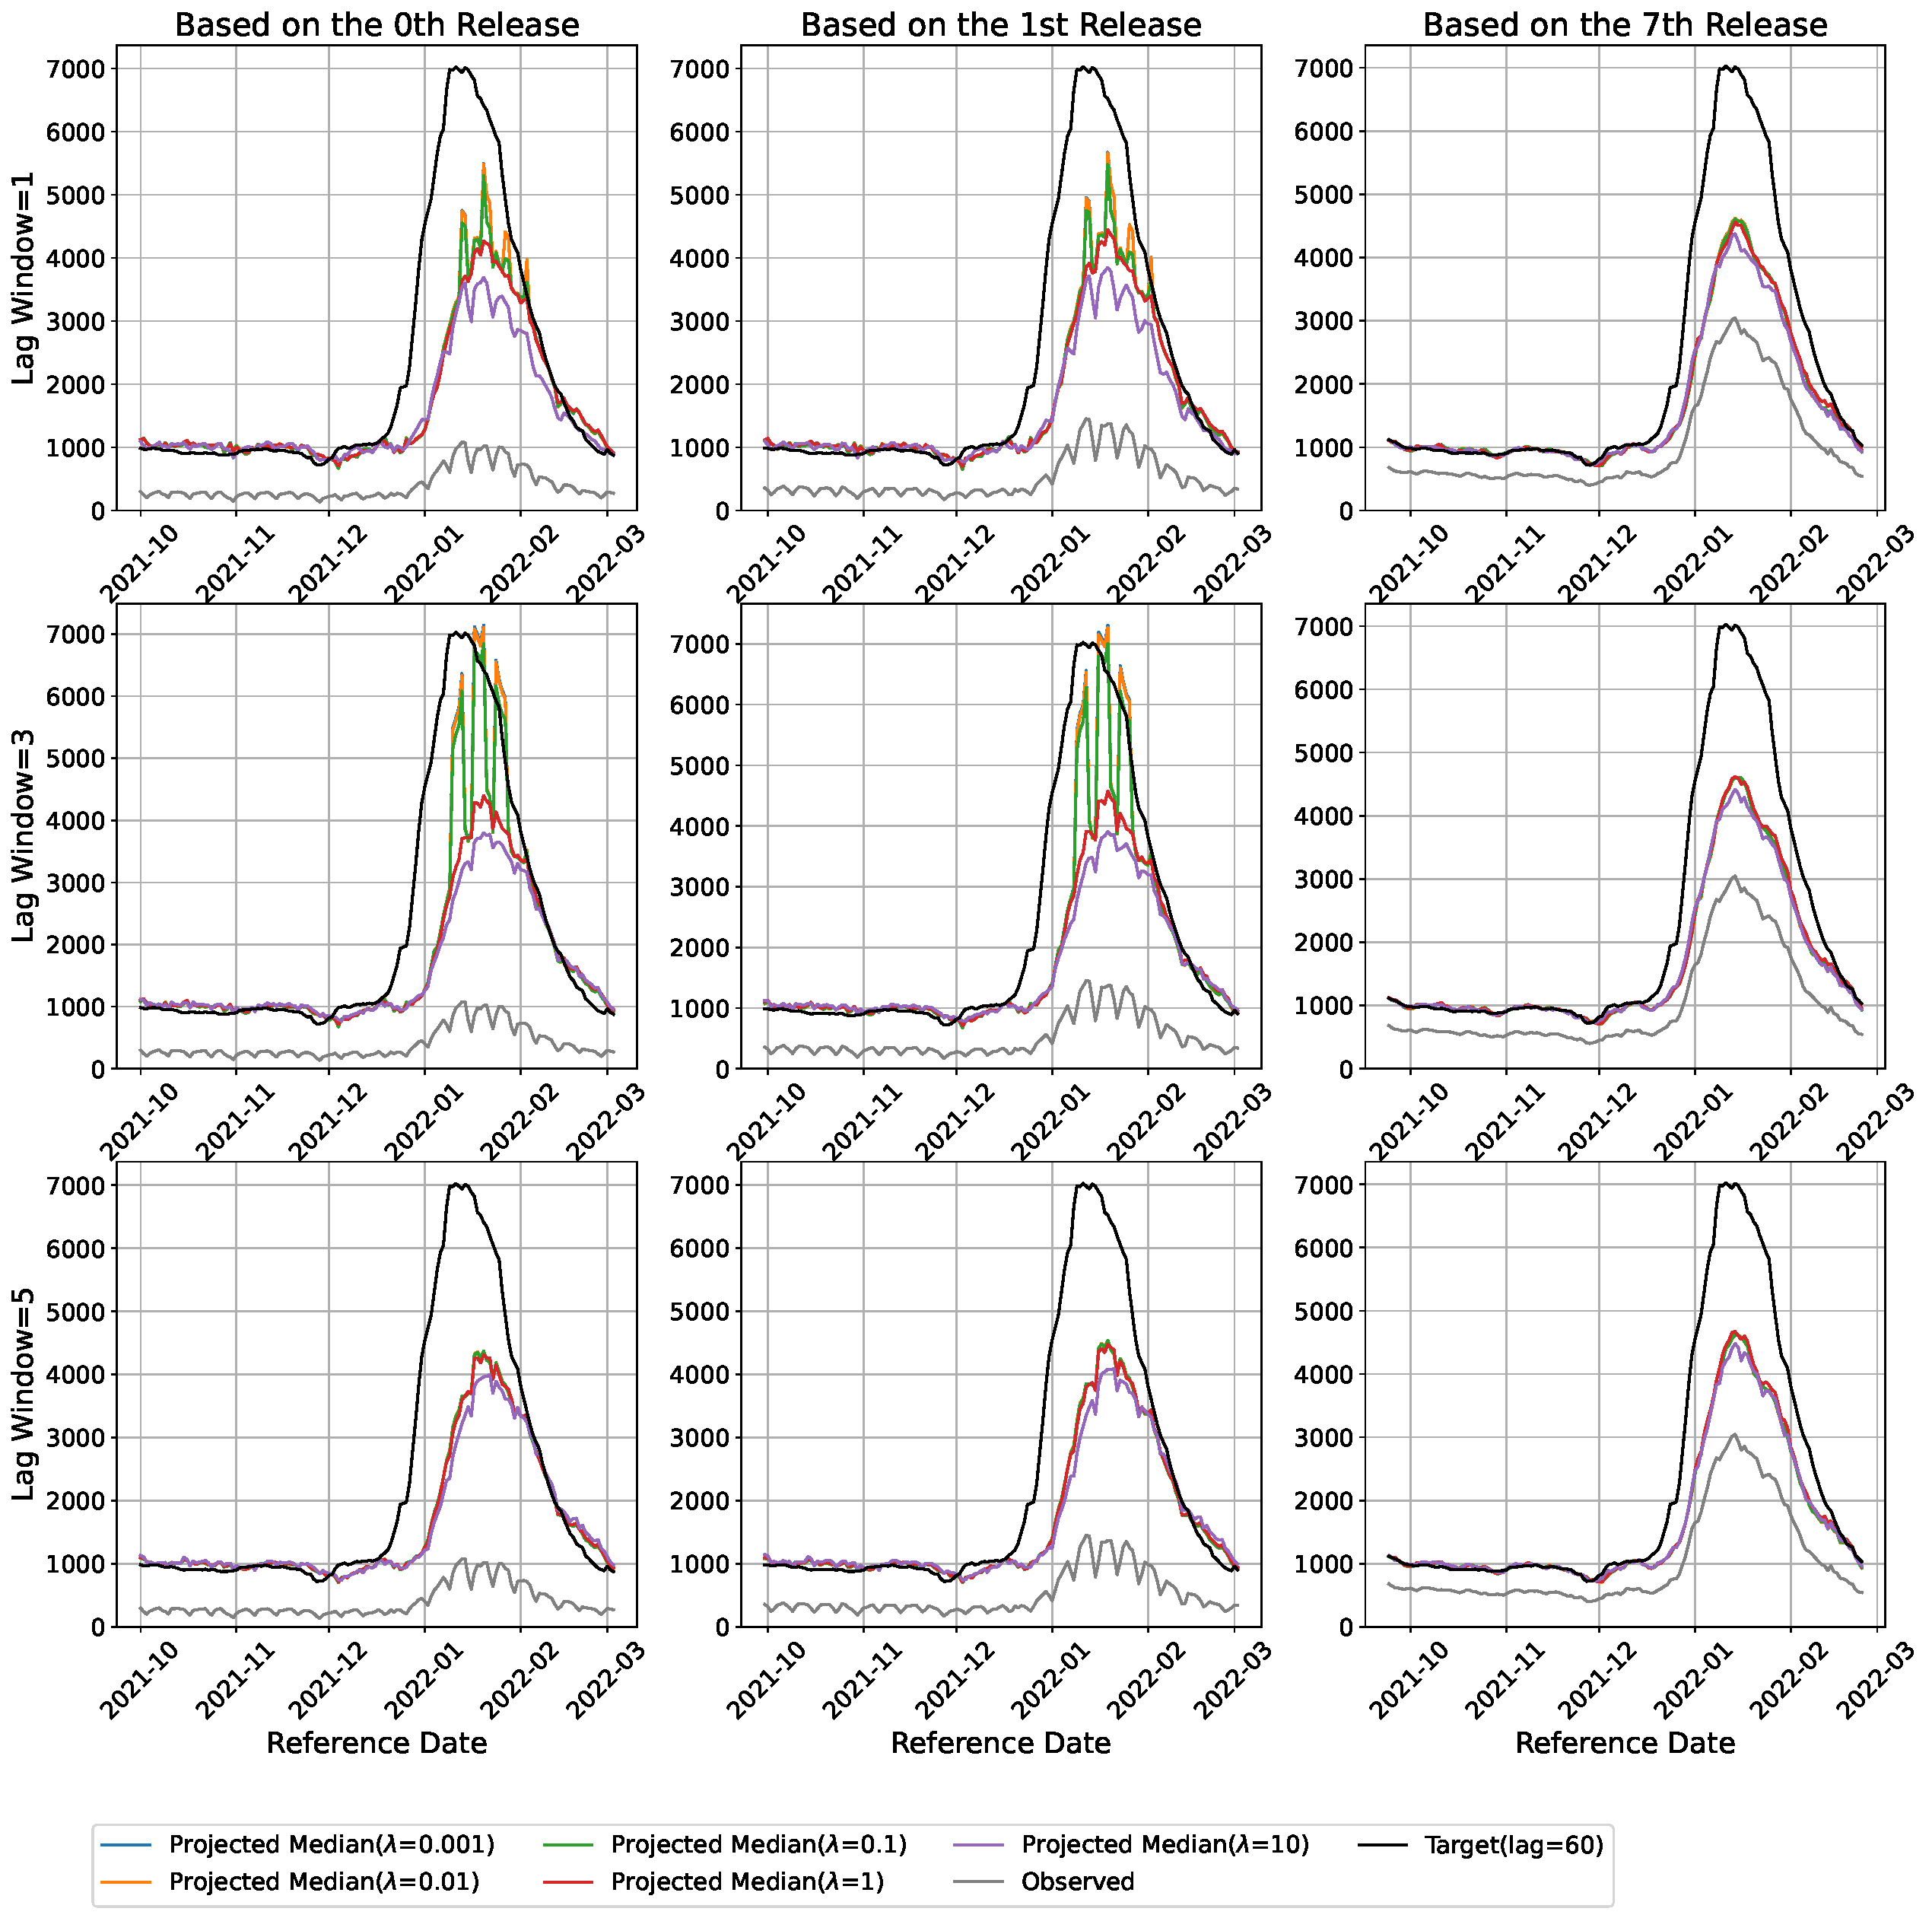
\includegraphics[width=\textwidth]{figs/count_pred_lambda_lagpad_tuning_ca_new_covs_added.pdf}
    \caption{\textit{}}
\end{figure}

\subsection{Incorporating Fraction Adjustment for Fraction Projection}
Turning our focus now to fraction projection. Different from counts projection where zeros are simply filled with missingness when there is no update provided yet, the edge cases for fraction projection is more complicated to dealing with. We mainly suffer from two cases: 1) fraction with extremely small denominators (can even be zeros) which means the revision of numerators is faster than that of denominators. This can result in incredibly large fraction observations. Such fractions are not statistically representative and mostly exist when lag is super small; 2) fraction equals to zero. The log transformation $f(\cdot)$ proposed in the previous section are no longer suitable for this case since fractions are already small enough. Inappropriately large constant $a$ can introduce noise into the data\cite{Bosse2023}. 

Here we propose a Beta prior approach based on a $\mbox{lag}^{-1}$ model, which can also serve as a baseline model. The make all the observations valid fractions, we add 1 and 100 respectively to the numerators and denominators beforehand. For location $i$, at test date $S$, consider the model below

$$Q_{f(Y_{itL})|f(X_{itl})}^{\tau}= \beta^{\tau T}X_{itl}$$

Covariates included in $X_{itl}$ are the following:

\begin{itemize}
    \item $\mathbbm{1}(\mbox{wd}(t+l) == k)$: indicator functions checking the day-of-week of the report date $t+l$, where $k \in \{0, 1, 2, ..., 5\}$. 
    \item $\mathbbm{1}(\mbox{wd}(t) == k)$ : indicator functions checking the day-of-week of the report date $t$, where $k \in \{0, 1, 2, ..., 5\}$.
    \item $\mathbbm{1}(\mbox{mw}(t+l) == k)$ : indicator functions checking the week-of-month of report date $t+l$, where $k \in \{0, 1, 2, ...,3\}$
    \item $f(\widetilde{y}_{itl})$: average of 7-day past values on log scale.

\end{itemize}

\begin{figure}
    \centering
    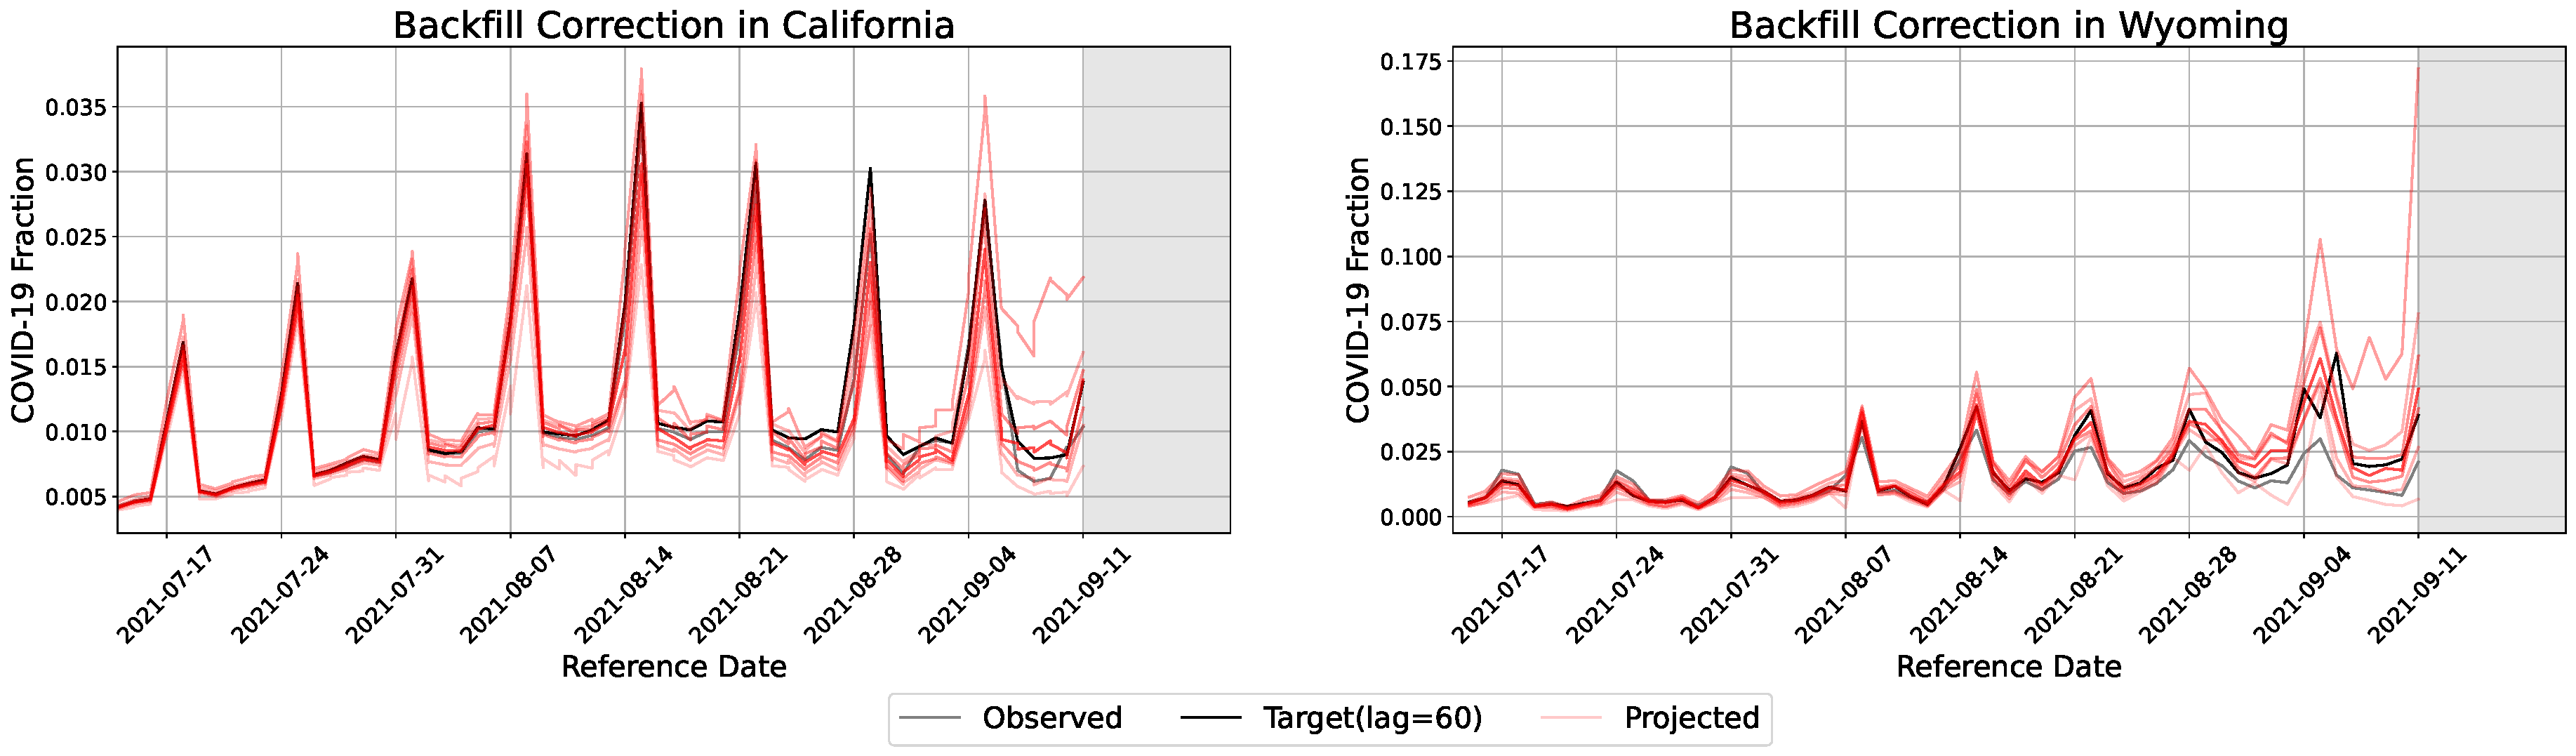
\includegraphics[width=\textwidth]{figs/fraction_pred_example_ca&wy.pdf}
    \caption{\textit{Illustration of estimating target of CHNG outpatient COVID-19 fractions as of 2021-09-11. The gray curve shows the most recent release of the COVID fractions based on CHNG outpatient data in California and Wyoming. The red lines show the projected quantiles of the 60th revision of the COVID-19 fractions for each reference date. The black curve shows the actual 60th revision for the values of each reference date in the future.
}}
\end{figure}

We assume that $Y_{itl}|X_{itl}$ follows Beta distribution that are day-of-week specific. For each day of a week, the predicted quantiles of $y_{itl}$ on log scale are exponentiated and utilized to estimate the parameters $\alpha$ and $\beta$ of the Beta distribution using Non-Linear Minimization\cite{Dennis1983}\cite{Schnabel1985}. And then,  
$$\mbox{Pseudo Numerator} = \alpha$$
$$\mbox{Pseudo Denominator} = \alpha + \beta$$
$$y_{itl} = \frac{\mbox{num}_{itl}}{\mbox{denom}_{itl}} \rightarrow \frac{\mbox{num}_{itl} + \alpha}{\mbox{denom}_{itl} + \alpha + \beta}$$
This adjustment is applied not only to $y_{itl}$ but also to all corresponding covariates. 



\section{Evaluation}

We now evaluate projection performance for all locations of interest (50 states and top 200 populous counties)  and for all test dates between 2021-08-30 and 2023-03-11 inclusive (589 days in total) against the target values as defined in section 2.1. To reiterate, in our real-time backfill correction experiment, we restrict our access to data that would have been available at each test date $S$. In order to save time computationally, we train the model for every 14 consecutive days but not daily. 

We use the weighted interval score(WIS) to evaluate the distance between the projected distribution and the target value. Suppose our projected values are notated as $\hat{Q}_{(Y_{itl})}(\tau)$ after exponentiation, which represents the projected $\tau$th quantile of $Y_{itL}$ given $y_{itl}$ and corresponding covariates. Notice that in the count projection, for each location $i$ and reference date $t$ pair, we have multiple data points with different lags to project the same $Y_{itL}$. To distinguish the projection results from these points, we will re-write them as $\hat{Y}_{itl}|X_{itl}$. Therefore, the WIS scores are calculated by comparing the distribution of $\hat{Y}_{itl}$ on log scale with the distribution $Y_{itL}$ on log scale no matter for counts or fractions. 

Figure X shows an example of count projection based on CHNG outpatient COVID claims in California. The real-time report, which will be revised in the next two months, largely deviates from the truth temporarily. In such cases, our model can avoid misjudgment of trends due to claims counts that are not reported in time. The distribution of fractions is much different from the previous one, and the pattern is more complicated since the revisions of the fractions are no longer monotonically increasing. 
%% Use projection for 7dav instead of daily
Figure X shows the example of fraction projection based on CHNG outpatient COVID-19 fractions in Harris County, TX. With only a limited number of revisions, the predictions provided by our model are close enough to the target values, which are available two months later after the first release. 

\begin{figure}
    \centering
    \includegraphics[width=\textwidth]{}
    \caption{\textit{}}
\end{figure}

To have a broad view of the projection performance, the projection errors are aggregated into an average on log scale and can be interpreted as the geometric average of relative error if exponentiated. The real-time observation can roughly serve as the projected median from a baseline model. For the purposes of making fair comparisons, we include the mean absolute error on log scale using the projected media




Test on other datasets:
choice 1) MA DPH : well known, but not available for all dates of interest (starting from 2021, 1, 4. End of 2022, 7, 8)
choice 2) Quidel Antigen Data
choice 3) CHNG Inpatient Data





\section{Discussion}
The curve of \%percent of reported counts over revisions indicates that specific backfill patterns exist. Quantification of such backfill patterns and the evaluation of projection results remains a challenge. We use weighted interval scores to evaluate our log-scale projection to investigate the relative errors which can vary broadly in different regions and time periods.  The current strategy is reasonable enough but not perfect. As shown in Figure X shows examples of poor projection performance for the locations with small target fractions. Minor absolute errors are magnified in the relative error evaluation system. We believe that he same relative error is less acceptable for areas with higher infection densities. 

%% TODO: Not the latest version.  
%% Use log 10 or natural log scale? natural log add the second axis? 
\begin{figure}
    \centering
    \includegraphics[width=\textwidth]{figs/evl_comparison_states.png}
    \caption{\textit{red lines represent the 10 states with the worst prediction performance while blue lines represent the 10 states with the best prediction performance}}
\end{figure}

Due to the exponential nature, situations in which models missed the beginning of upswings are more strongly emphasized while failing to predict a downturn following a peak is less severely penalized. 
\begin{figure}
    \centering
    \includegraphics[width=\textwidth]{figs/pred_problem_in_ca.pdf}
    \caption{\textit{the backfill correction}}
\end{figure}

\begin{figure}
    \centering
    \includegraphics[width=\textwidth]{figs/new_covs_zoom_in.pdf}
    \caption{\textit{the backfill correction}}
\end{figure}
\section{Acknowledgements}
The authors are grateful to Aaron Rumack, Roni Rosenfeld, Bryan Wilder, Ryan Tibshirani, Logan Brooks, Will Townes for insightful conversations. 
This work was supported by the fellowship from the Center for Machine Learning and Health at Carnegie Mellon. 



\clearpage

\printbibliography
\end{document}